%\documentclass[openright,twoside,headsepline]{scrbook}
%\usepackage[applemac]{inputenc}
%\usepackage{graphicx,xcolor,hyperref} % obsolete in HU-diss
%\usepackage[round,authoryear]{natbib}
%\setlength\bibhang{2em} 
%
%
%\KOMAoptions{numbers=noenddot}
\usepackage{amsmath,amssymb,amsfonts,amsthm,epigraph,scrpage2}
\usepackage[ngerman,english]{babel}
\definecolor{Cayenne}{rgb}{0.502,0.0,0.0}
\definecolor{Steel}{rgb}{0.4,0.4,0.4}


%\setcounter{secnumdepth}{3} % sub subsections numbering
%\setcounter{tocdepth}{3} % subsubsections inTOC

\usepackage[format=plain,singlelinecheck=false, font={sf,small},labelfont={bf,color=Steel}]{caption}
\DeclareCaptionLabelSeparator{cayenne_period}{\textcolor{Cayenne}{.} }
\captionsetup{labelsep=cayenne_period}

% Colors
\addtokomafont{chapter}{\color{Steel}}
\addtokomafont{section}{\color{Steel}}
\addtokomafont{subsection}{\color{Steel}}
\addtokomafont{subsubsection}{\color{Steel}}
\addtokomafont{paragraph}{\color{Steel}}

\addtokomafont{pagehead}{\color{Steel}}
\renewcommand{\pnumfont}{\color{Steel}} 
\addtokomafont{headsepline}{\color{Steel}} 
\pagestyle{scrheadings} 

%\makeatletter % dot after sections and all below
%\let\std@sect\@sect
%\def\@sect#1#2#3#4#5#6[#7]#8{\std@sect{#1}{#2}{#3}{#4}{#5}{#6}[#7.]{#8\color{Cayenne}{.}}}
%\makeatother

\usepackage[leftcaption]{sidecap} % inner, outer,left,right
\sidecaptionvpos{figure}{t}

% Papiergr��e
%\setlength{\paperwidth}{24cm}
%\setlength{\paperheight}{17cm}
%\recalctypearea
%\usepackage{geometry}

%% Flattersatz
%\usepackage[document]{ragged2e} % Flattersatz
%\setlength{\RaggedRightParindent}{1em} % evtl. parskip


%% Sans Serif
%\usepackage{cmbright}
%\renewcommand{\familydefault}{\sfdefault}
%% Palatino
%\usepackage[sc]{mathpazo}
%\linespread{1.05}         % Palatino needs more leading (space between lines)
%\setkomafont{sectioning}{\normalcolor\bfseries} % Kapitel�berschriften

%%% Kapitel�berschriften: Mit gro�en Zahlen
%\usepackage{titlesec}
%\titleformat{\chapter}[display]
%{\bfseries\Large}
%{ %\Huge\textsc{\chaptertitlename} % f�r das Wort 'Kapitel'
%\hfill\fontsize{120}{70}\selectfont\color{lightgray}\textbf{\thechapter}}
%{-2ex}
%%{\filleft\fontsize{50}{70}\selectfont\scshape} % Kapit�lchen oder...
%{\filleft\fontsize{50}{70}\selectfont\textbf} % ...oder keine Kapit�lchen
%[\vspace{0ex}]
%
%%%% Part�berschriften
%\titleformat{\part}[display]
%{\bfseries\Large}
%{ %\Huge\textsc{\chaptertitlename} % f�r das Wort 'Kapitel'
%\hfill\fontsize{120}{70}\selectfont\color{lightgray}\textbf{\thepart}}
%{-2ex}
%{\filleft\fontsize{50}{70}\selectfont\scshape} % Kapit�lchen oder...
%%{\filleft\fontsize{50}{70}\selectfont\textbf} % ...oder keine Kapit�lchen
%[\vspace{0ex}]


\newcommand{\ER}{Erd\H{o}s-R\'enyi }
\newcommand{\BA}{Barab\'asi-Albert }
\newcommand{\mean}[1]{\left< #1 \right>}
\newcommand{\abs}[1]{\left| #1 \right|}
\newcommand{\norm}[1]{\lVert#1\rVert}
\newcommand{\mat}[1]{\mathbf{#1}}
\newcommand{\tgraph}{\mathcal{G}}

\theoremstyle{definition} % non-italic
\newtheorem{annahme}{Annahme} % braucht amsthm
\newtheorem{definition}{Definition}
\newtheorem{theorem}{Theorem}
\newtheorem{satz}{Satz}
\newtheorem{frage}{Frage}
%\input{watermarks/watermark.tex}
\DeclareMathOperator{\nnz}{nnz}

% + Graphicspath nach begin document

%
%
%
%\begin{document}
%\graphicspath{{/Users/lentz/Documents/GitHub_locals/Thesis/images/}}
%\tableofcontents

\chapter{Appendix}

\section{Network implementation}\label{sec:implementation}
In order to efficiently implement networks and their analysis on a computer, it is necessary to use appropriate data structures.
A short and transparent introduction to data structures and algorithms is in the book of \citeauthor{algorithm_design} \citep{algorithm_design}.
In this section, we review some essential data structures appropriate for network analysis and give a brief description of fundamental algorithms.
The purpose of this section is to sketch the basic ideas behind the data structures and algorithms rather than to list algorithms and source code.
For source code of data structures and algorithms, the reader is encouraged to the lecture of \citep{algorithm_design} and \citep{Merali:2010ih}.

\paragraph{Matrix implementation\color{Cayenne}{.}}
To begin with, we consider the implementation of adjacency matrices as introduced in section \ref{sec:network_matrices}.
%Matrices can be seen as a \emph{graph centric view} on the network, since they map the whole network topology onto a single object.
Adjacency matrices are by definition square matrices.
Their entries are either $0$ or $1$.
In weighted networks, their entries can take any floating-point value.
The number of nodes in most complex network datasets is relatively large. 
Starting with small networks (100 nodes, conference contacts \citep{isella2011}), complex networks can be gigantic ($\sim 10^9$ nodes in the case twitter tweeds \citep{Yang:2011} or the world-wide web \citep{Albert:1999uu,Broder:2000ej})
Note that the sizes of adjacency matrices scales with the square of the networks size, hence adjacency matrices of these networks are intractable for straightforward computer-based matrix analyses.

Nevertheless, it is a common feature of many real-world networks that they are sparse, i.e. the vast majority of their entries are zeros\footnote{Typically, the number of edges in the network is of the same order as the number of nodes.}.
Since zeros do not contribute to matrix operations as products or additions, it is reasonable to use data structures ignoring zeros.
These data structures are called \verb"sparse matrices".
Their advantages is (1) they save much memory and (2) computations are faster, because operations with zeros involved are not executed.
Sparse matrix data structures are available in most modern computer languages (e.g. Matlab, Python: \verb"scipy" library, C/C++: \verb"boost" library).
They perform well for problems based on adjacency matrices as the computation of the degree or eigenvector centrality.
However, matrix methods are not suitable for the computation of many other network measures, such as betweenness, closeness or network navigation.

\paragraph{Graph implementation\color{Cayenne}{.}}
The drawback of matrix representations of networks is that it is rather complicated to \emph{traverse} a network using matrices.
A traversal is a procedure of the following form: start at a node, visit all of its neighbors, from each neighbor visit its neighbor and so forth, until there are no more new nodes to traverse.
This is a searching process.
Network traversal is used in many implementations of graph theoretic methods.

As an alternative implementation of the adjacency matrix the \verb"adjacency list" is a well suited data structure for network traversal.
It stores the neighbors of every node and can be implemented as linked lists.
Adjacency lists can be considered as a node centric view on the network, since they allow for a fast access to the neighborhood of each node.
Considering the example network on the left panel of Figure~\ref{fig:dfs_bfs}, the corresponding adjacency list is as follows:
\begin{align*}
1 &\rightarrow 2,3 \\
2 &\rightarrow 4 \\
3 &\rightarrow 2 \\
4 &\rightarrow 2,3 .
\end{align*}
In order to traverse the graph starting at node $1$, we choose one of the neighbors of $1$ and repeat the process until we have traversed all nodes.
One possible traversal starting at $1$ would be $1\rightarrow 3 \rightarrow 2 \rightarrow 4$.

During a traversal process, one can decide to either exploit the whole neighborhood of a node first and then traverse the next generation or choose a neighbor of every traversed node at every step.
These two essential searching processes are called breadth-first-search (BFS) and depth-first-search (DFS), respectively.
The difference between the two lies in the order of traversed nodes.
Figure \ref{fig:dfs_bfs} shows resulting search trees of the two methods.
Starting at node $1$, the traversal $1\rightarrow 3 \rightarrow 2 \rightarrow 4$ would be found using a DFS-search, while a BFS-search would yield $1\rightarrow 2 \rightarrow 3 \rightarrow 4$.
It should be noted that in general there exist multiple BFS and DFS trees for each starting node. 
%
\begin{figure}[htb]
\begin{center}
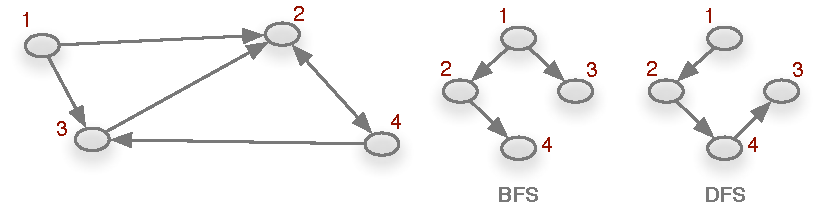
\includegraphics{DFS-BFS.pdf}
\caption{Breadth-first-search and depth-first-search trees in a directed network. Search processes are started at node $1$.}
\label{fig:dfs_bfs}
\end{center}
\end{figure}

Both search algorithms are used in a large number of algorithmic applications.
BFS is efficient to compute shortest paths in unweighted networks.
With every generation in a BFS tree, the distance from the starting node is incremented by 1, and thus the set of nodes with a certain distance from the starting node can be directly read from the BFS tree (see Figure~\ref{fig:dfs_bfs}).
Shortest paths in weighted networks can be identified using a the algorithm of Dijkstra \citep{Dijkstra:1959}.
Connected components in directed graphs can be efficiently identified using closed DFS paths \citep{algorithm_design}.

Due to the sparsity of typical adjacency matrices, networks can also be efficiently stored as \verb"edge lists".
An edge list is a list of tuples, where each tuple $(u,v)$ is an edge connecting nodes $u$ and $v$.
The edge list of the network shows in Figure~\ref{fig:dfs_bfs} is
\begin{align*}
&(1,2)\\
&(1,3)\\
&(2,4)\\
&(3,2)\\
&(4,2)\\
&(4,3) .
\end{align*}
Due to their human readable structure, edge lists are a convenient format to store networks as column wise text files.
Edge lists can also be efficiently used for edge randomization and random graph generation.

Implementations of the graph structures discussed above are for example available in the libraries \verb"networkx" (Python), \verb"igraph" (C, Python, R), \verb"Lemon" and \verb"Boost" (C++).

\paragraph{Hard problems\color{Cayenne}{.}}
The tools introduced above provide a huge and efficient toolbox for network analysis.
Nevertheless, there are still network problems, where no efficient algorithm is known for their exact solution.
In the language of complexity theory, the time to solve these problems scales with the problem size in non-polynomial time.
There are two important complexity classes of problems in computational complexity theory.
First, the class of NP-complete (NP stands for Non-deterministic Polynomial-time) problems, and second, the class of NP-hard problems.
All problems mentioned in this thesis have been proven to be NP-complete in our context.
For most practical questions, a distinction between the two classes is irrelevant, however.
It is rather important to recognize intractable graph theoretical problems.
NP complete problems can typically be solved exactly only for small system sizes.

Probably the most popular example is the \emph{traveling salesman problem}: a salesman has to traverse a set of cities and thereby choose the order of those cities that minimizes the total distance.
For small problem sizes, it is possible simply to try out all possible combinations and find the minimal total distance (brute-force search).
The number of possible combinations, however, grows factorial with the system size, i.e. finding a solution takes $t\propto n!$ for $n$ cities.
In other words, if the problem could be solved for 20 cities in 1 second, it would take 21 seconds to solve it for 21 cities, 7 minutes for 22 cities and 3 million years for 30 cities!

A more exhaustive overview about hard problems is in \citep{algorithm_design} and the references therein.
Generally, heuristic methods have to be used in order to get an approximate solution.
It should be noted that the \emph{maximum clique} problem (see section \ref{sec:PRL}) and \emph{graph partitioning} (see section \ref{sec:network_analysis}, Equation~\eqref{eq:modularity}) belong to the class of hard problems \citep{brandes2007}.

\section{Degree vs. other centrality measures}\label{sec:centrality_hit}
In this section, we compute the centrality measures introduced in Section~\ref{sec:micro_measures} and compare them with the degree.
In particular, we compare the degree with betweenness, closeness and eigenvector centrality.
Since the eigenvector centrality is defined only on connected networks, the analysis is restricted to the LSCC of the network.
%
\begin{figure}[htb]
\begin{center}
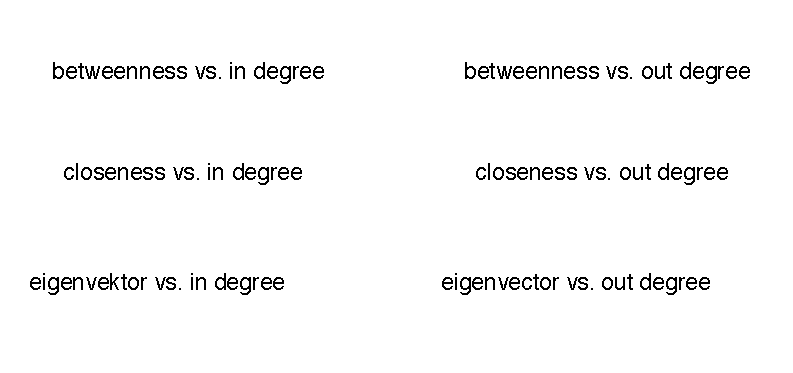
\includegraphics{static_centrality_pvm.pdf}
\caption{Correlation between the degree and other centrality measures for the livestock trade network.
The left panel shows the closeness centrality $C_C$, eigenvector centrality $C_E$ and betweenness centrality $C_B$ vs. the in-degree.
The respective picture for the out-degree is shown on the right.
Dashed lines show power-law fits of the data.
Only nodes with in/out-degree greater than 10 are shown.}
\label{fig:centrality_pvm}
\end{center}
\end{figure}
%
Figure~\ref{fig:centrality_pvm} shows different centrality measures for the network being compared with the degree.
Each point represents one node, and the dashed lines show power-law fits of the scatter plots, respectively.
The figure demonstrates that all considered centrality measures show a correlation with the the degree.

\section{Subgraphs and maximum modularity}\label{sec:maximum_modularity_subgraphs}
Although computer generated modular networks are used in many applications, the author is not aware of any systematic analysis of the maximum value of modularity depending on the number of modules.
Therefore, we derive an estimation of the maximum modularity value depending on the number of modules in the network.
The results are derived for a clique of modules, but remain unchanged for a ring of modules as this distinction is reasonable in finite systems.
In addition, the estimation is also valid for directed networks.

The modularity of a network with given modular structure can be computed using the equation
\begin{equation}\label{eq:mod_undir}
Q=\sum _i \left( e_{ii}-a_i^2 \right),
\end{equation}
where $e_{ij}$ is the fraction of edges pointing from community $i$ to community $j$.
The last term corresponds to the fraction of all edges that are connected to community $i$, i.e.
\[
a_i = \sum _j e_{ij}.
\]
Since the sum over all edge fraction has to be 1, it is $\sum _{ij}e_{ij}=1$.
If a network consists of two modules $x$ and $y$, the fraction of edges in $y$ is
\begin{equation}\label{qmaxbedingung}
y=c-x,
\end{equation}
where the constant $c<1$ is the fraction of all inner module edges.
In general, this expression is $c=\mathrm{Tr} (e)$.

\subsection{Two modules}
In the case of two communities, the fraction of inter-module-edges is uniquely determined by the fraction of inner-module-edges.

The matrix $e_{ij}$ takes the form
\[
e_{ij}=\left(\begin{array}{cc}x & \frac{1}{2}(1-x-y) \\ \frac{1}{2}(1-x-y) & y\end{array}\right) ,
\]
where $x$, $y$ are the edge fractions \emph{in} communities 1 and 2 and $\frac{1}{2}(1-x-y)$ is the fraction of edges \emph{between} communities 1 and 2.
The corresponding expression for $Q$ is.
\[
Q=x-\left( x+\frac{1-x-y}{2} \right) ^2 +y -\left( y+\frac{1-x-y}{2} \right) ^2 .
\]
This function does not possess a maximum over the total domain, but there is a maximum in the subdomain $0<x<1$, $ 0<y<1$.
Condition \eqref{qmaxbedingung} yields
\[
Q=\frac{1}{2}+2\, cx-2\, x^2-\frac{1}{2}\, c^2+c.
\]
Using condition \eqref{qmaxbedingung} restricts the function to tuples $(x,y)$, where $x+y=c$, which corresponds to a line $y=c-x$.
Thus, we are looking for the maximum along this line using the condition
\[
\frac{\partial Q}{\partial x}=2c-4x=0.
\]
It follows $x=c/2$ and the maximum condition $\partial ^2 Q/\partial x^2 =-4<0$ is satisfied.
Using \eqref{qmaxbedingung} gives the solution
\begin{equation}\label{qmax_xy}
x=\frac{c}{2} , \hspace{0.5cm} y=\frac{c}{2}.
\end{equation}
The corresponding modularity is 
\begin{align*}
Q&=\frac{c}{2}-\frac{1}{4}\left( 1+\frac{c}{2}-\frac{c}{2} \right) ^2 +\frac{c}{2}-\frac{1}{4}\left( 1+\frac{c}{2}-\frac{c}{2} \right) ^2 \\
&= c- \frac{1}{2} .
\end{align*}
The case where a maximum fraction of edges is in the modules and a minimum fraction is between modules is met, if $c\rightarrow 1$.
In this case, the modularity takes its maximum value.
The limit is
\begin{equation}\label{q2limits}
\lim _{c\rightarrow 1} x =1/2, \hspace{0.5cm}\lim _{c\rightarrow 1} y =1/2, \hspace{0.5cm} \lim _{c\rightarrow 1} Q=1/2.
\end{equation}
For the case of two modules, the maximum modularity is found for two equally sized modules of approximate size $1/2$.
The maximum modularity is then $Q=0.5$.
We consider the case of more modules below.

%
\subsection{Arbitrary number of modules}
In the case of more than two modules, all modules can have different sizes in the first place and can be connected among themselves arbitrarily.
The general module-matrix takes the form
\begin{equation}\label{eq:general_module_matrix}
e_{ij}=\left(\begin{array}{ccccc}x_1 &  & \hdots &  & d \\ & x_2 &  &  &  \\\vdots &  & \ddots &  & \vdots \\ &  &  & \ &  \\d &  & \hdots &  & x_n\end{array}\right) .
\end{equation}
All non-diagonal elements are 
\[
d= \frac{1-\text{Tr } (e) }{n(n-1) } = \frac{1-c }{n(n-1) }
\]
with $c\equiv \text{Tr } (e)=\text{const.}<1$.
Thus, the general expression for modularity is
\begin{equation} \label{eq:modumatrix}
Q= c-\sum  _i \left( \sum _j e_{ij} \right)^2 .
\end{equation}
%
We use the above expression for the non-diagonal elements $d$ and compute the expression $\sum _j e_{ij}$ in Equation~\eqref{eq:modumatrix}.
\begin{equation}\label{eq:sumeij}
\sum _j e_{ij} = e_{ii} + \sum _{j\neq i} e_{ij} = x_i + (n-1) \frac{1-c}{n(n-1)} = x_i + \frac{1-c}{n}.
\end{equation}
%
Now we insert $\sum _j e_{ij}=x_i+\frac{1-c}{n}$ in Equation~\eqref{eq:modumatrix} and after some algebra we get a general expression for the modularity for networks of the form \eqref{eq:general_module_matrix}:
\begin{equation}\label{eq:Qndim}
Q=c-\sum _i x_i^2 - \frac{1-c^2}{n} = \sum _i x_i -\sum _i x_i^2 - \frac{1-(\sum _i x_i)^2}{n}.
\end{equation}

In order to find the relevant maximum of \eqref{eq:Qndim}, its slope has to vanish along a hyperplane defined by
\begin{equation}\label{qmehrdimbedingung}
\sum _i x_i = c = \text{const.} <1.
\end{equation}
%
Since $c$ is constant, the relevant part of \eqref{eq:Qndim} for the maximum is
\begin{align}
Q_{\text{relevant}}\equiv Q_\text{r}= -\sum _{i=1}^n x_i^2&=-\sum _{i=1}^{n-1} x_i^2- \underbrace{ \left( 
c-\sum _{i=1}^{n-1} x_i \right) ^2 }_{x_n^2} \label{eq:relevant_Q}\\
&= -\sum _{i=1}^{n-1} x_i^2 - c^2 + 2c\sum _{i=1}^{n-1} x_i -\left( \sum _{i=1}^{n-1} x_i \right) ^2. \nonumber
\end{align}
Note that the sum on the right-hand side is up to $n-1$.
This effectively eliminates the last variable.
The derivative of $Q$ is
\begin{equation}
\frac{\partial Q}{\partial x_i}= \frac{\partial Q_\text{r}}{\partial x_i}=- 2\sum _{i=1}^{n-1} x_i + 2c(n-1)-2 (n-1) \sum _{i=1}^{n-1} x_i.
\end{equation}
%
In order to find a maximum, the derivative has to vanish, i.e.
\begin{align*}
0&=- 2\sum _{i=1}^{n-1} x_i + 2c(n-1)-2 (n-1) \sum _{i=1}^{n-1} x_i \\
&=- \sum _{i=1}^{n-1} x_i + c(n-1) - (n-1) \sum _{i=1}^{n-1} x_i \\
 &= cn-c-n\sum _{i=1}^{n-1} x_i +\sum _{i=1}^{n-1} x_i -\sum _{i=1}^{n-1} x_i\\
 &= cn-c-n\sum _{i=1}^{n-1} x_i .
\end{align*}
It follows
\[
\underbrace{c-\sum _{i=1}^{n-1} x_i}_{x_n} =\frac{c}{n}.
\]
Thus,
\begin{equation}
x_n=\frac{c}{n}.
\end{equation}
Hence, the maximum of $Q$ is obtained, if all modules have the same size, i.e. $x_i=\frac{c}{n} \; \forall i$.

In order to find the maximum value of $Q$, we insert the module size $x_i=c/n$ into Equation~\eqref{eq:Qndim} and get
\[
Q=c-\sum _{i=1} ^n \left( \frac{c}{n} \right) ^2 - \frac{1-c^2}{n}=c-\frac{c^2}{n}-\frac{1}{n}+\frac{c^2}{n}.
\]
Thus, it follows for dense modules
\begin{equation}\label{eq:q_max}
Q_\mathrm{max}= \lim _{c\rightarrow 1}Q=1-\frac{1}{n}.
\end{equation}
Consequently, the maximum value of $Q_\mathrm{max}$ is determined by the number of modules.
A similar result was found using probabilistic arguments in \citep{Good2010}.

\paragraph{Finite systems\color{Cayenne}{.}}
In finite systems, the minimum fraction of inter-module edges is obtained, when modules are connected to each other on a ring, each module having two nearest neighbors.
In this case we set  $e_{ij}= \frac{1}{n}(1-c)$ for $j=i+1$ and $j=i-1$ and all other elements are zero.
This yields
\begin{equation}\label{eq:ring_module_matrix}
e_{ij}=\left(\begin{array}{cccccc}
x_1 & \frac{1}{n}(1-c)&  & \hdots &  & 0 \\ 
\frac{1}{n}(1-c)& x_2 &\frac{1}{n}(1-c)&  &  &  \\
 & \frac{1}{n}(1-c) & \ddots & \ddots & & \\
\vdots &  & \ddots & \ddots & \ddots &\vdots \\
 & & & \ddots   &  x_{n-1} &\frac{1}{n}(1-c) \\
0 & &  & \hdots & \frac{1}{n}(1-c) & x_n
\end{array}
\right) .
\end{equation}
It follows immediately that $\sum _j e_{ij}=x_i+\frac{2(1-c)}{n}$, which is equivalent to \eqref{eq:sumeij} up to a factor 2.
Inserting this into Equation~\eqref{eq:modumatrix} gives a similar expression for modularity \eqref{eq:Qndim} as for the general case:
\begin{equation*}
Q=c-\sum _i x_i^2 - \frac{4(1-c)}{n} .
\end{equation*}
Since the relevant part for maximum finding is the quadratic term as in \eqref{eq:relevant_Q}, the results remain unchanged for modules along a chain and the maximum value is as above
\begin{equation}\label{eq:q_max2}
Q_\mathrm{max}=1-\frac{1}{n}.
\end{equation}

Figure~\ref{fig:q_max} shows a comparison between Equation~\eqref{eq:q_max2} and a computer simulation of a ring of modules where new modules are added to the system successively and the maximum modularity is computed. 
The edge density of each module is given by the edge occupation probability $p_\mathrm{in}=0.5$.
The figure demonstrates that Equation~\eqref{eq:q_max} gives a good approximation of the maximum value $Q_\mathrm{max}$ even for small systems.
%
\begin{SCfigure}
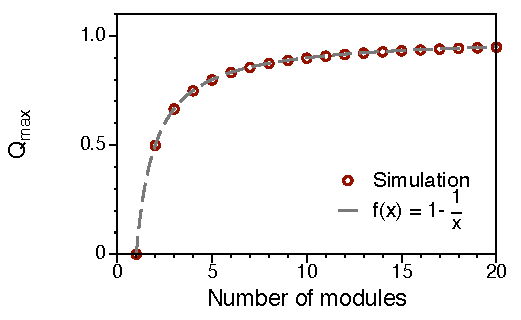
\includegraphics{Q_max.pdf}
\caption{Equation \eqref{eq:q_max2} (grey dashed line) reproduces the values found by numerical simulations (red circles).
In the simulations, modules are dense, directed subgraphs ($p_\mathrm{in}=0.5$) with $32$ nodes each.
Modules are connected on a ring so that the resulting graph is connected.
}
\label{fig:q_max}
\end{SCfigure}

\paragraph{Directed networks\color{Cayenne}{.}}
In analog to Equation~\eqref{eq:mod_undir} the modularity of directed networks can be written as \citep{Kao:2007}
\begin{equation}\label{eq:mod_directed}
Q=\sum _i e_{ii} - a_i ^{\text{in}} a_i ^{\text{out}}.
\end{equation}
where
\[
a_j ^\text{in}= \sum _i e_{ij} \hspace{1cm} \text{and} \hspace{1cm} a_i ^\text{out}= \sum _j e_{ij}.
\]
The structure of the inter-module edges takes the form of the matrix \eqref{eq:ring_module_matrix} and thus results do not differ either for the directed case.






%
%\bibliographystyle{apalike}
%\bibliography{/Users/lentz/Documents/GitHub_locals/Thesis/bibliography.bib}
%\end{document}
%
